% !TeX spellcheck = en_US
\chapter{Introduction}\label{ch:introduction}

This chapter first gives the context of the thesis and introduces the research problem the thesis addresses. Furthermore, this chapter discusses the research questions the thesis is trying to answer and what approaches the thesis adopts to investigate these questions.

\section{Background}\label{sec:introduction:background}

\glspl{amr} have gained enormous significance in automated factories. Recent developments in robotics and \gls{ai} have enabled the \gls{amr} to operate with autonomy. This requires the \glspl{amr} to run computation- and memory-intensive algorithms related to image processing, path planning, \gls{slam}, and learning \cite{Saeik2021}. However, \citeauthor*{Baxi2022} point out this poses a challenge for the robot's onboard system, which has limited computational capabilities due to size and cost limitation as well as battery life. Furthermore, these algorithms are time-sensitive and can cause operational failure for the \glspl{amr} if the latency restrictions cannot be satisfied. It becomes essential for large automated factories using \glspl{amr} to address this problem. 

% Maybe mention Human-Robot Collaboration?

\begin{figure}[htb]
    \centering

    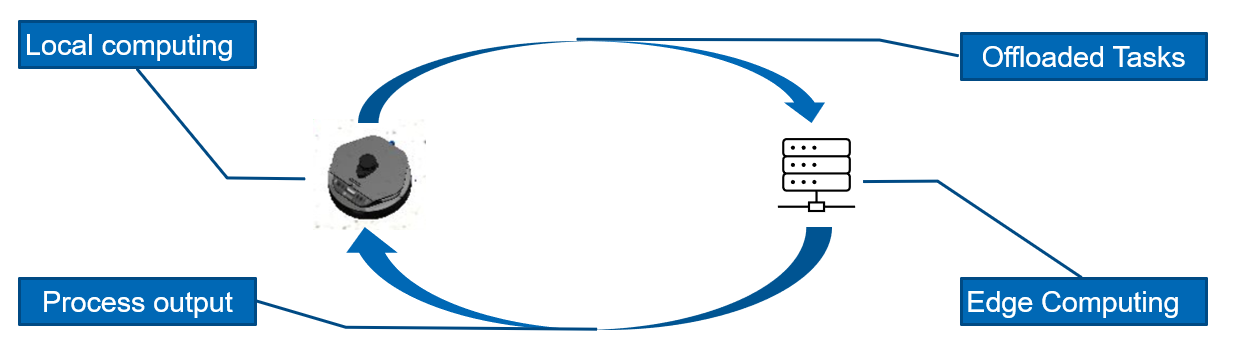
\includegraphics[width=120mm]{figures/setup/amr_offloading.png}
    \caption{Offloading pipeline between \gls{amr} and edge computer}

    \label{fig:amr_offloading}
\end{figure}

\gls{mec} as an evolution of \gls*{mcc} brings application hosting from data centers down to the edge of the network, where the data were initially collected, to achieve low latency and bandwidth efficiency \cite{Lin2019}. For latency-sensitive tasks on \glspl{amr}, such as perception and navigation, \gls{mec} offers an opportunity to enable the \glspl{amr} with limited resources by offloading costly computation tasks to the edge, while only a small portion of the computation remains on the \gls{amr}'s on-board system. A full offloading pipeline for \glspl{amr} is illustrated in figure~\cref{fig:amr_offloading}.


However, depending on the application scenarios, offloading certain tasks from the \glspl{amr} to the edge at all times may not be possible, beneficial or even feasible due to the network's latency, dynamic network changes, and resource availability. \citeauthor*{Baxi2022} point out that a simple perception task using an RGB-D camera can cause over 100 ms sensing-to-actuation round-trip latency and over 50 MBytes per second network bandwidth usage. On the other hand, offloading computational workloads to the edge could also impact the \gls{amr}'s safety, availability as well as on-board resources. The exact influence on the robotic system will depend on the chosen offloading strategy. Therefore, it is necessary to investigate the effects of certain offloading strategies on the \gls{amr}'s safety, availability, and task performance.

\section{Research Questions}\label{sec:introduction:research_questions}

This thesis first implements an offloading framework for robot perception and analyzes the effects of different offloading strategies, using \gls{ros} \cite{Macenski2022}. More specifically, this thesis considers a 2D object detection task using YOLOv5 network, proposed by \citeauthor*{Jocher2020}. YOLOv5n, a smaller variant of the perception network, will be deployed on the \gls{amr}'s on-board system, while the edge counterpart uses a more accurate but also more complex variant, e.g., YOLOv5l. The environment is an industrial warehouse containing human objects as obstacles. The \glspl{amr} are equipped with camera sensors and use the native \gls{ros} navigation stack, proposed by \citeauthor*{Macenski2020} to navigate from a user-defined route. 

This thesis first investigates offloading strategies with different offloading ratios. The \gls{amr} offloads a portion of the incoming frames from the camera to the edge computer with different offloading ratios incrementing from 0 percent to 100 percent with a stepping of 10 percent, i.e., the \gls{amr} offloads 10, 20, ..., 80, 90 percent of the incoming frames to the edge computer. At 0 percent, the \gls{amr} does not offload at all to the edge computer and only relies on its onboard resources. At 100 percent, the \gls{amr} does not perform any local computation and only relies on the computation output of the edge computer. This step aims to investigate the influence of different offloading strategies on the performance of the perception task and the resource usage of the \gls{amr} and the edge computer as well as the network. Then, this thesis carries on to implement a decision-making offloading strategy depending on run-time parameters, such as latency and \gls{amr}'s CPU usage and power consumption. This strategy is a simplified variant of the algorithm proposed by \citeauthor*{Ning2019} with a goal of minimizing latency and additional constraints subjected to power consumption and network bandwidth. 

This thesis evaluates the aforementioned offloading strategies regarding different metrics such as the CPU usage and power consumption of the \gls{amr}, the network bandwidth in use, and the mean average precision of the 2D object detection algorithm for human obstacles. The offloading strategies are first evaluated in simulation and later on in real robotic systems. With the results from these experiments, this thesis is trying to answer the following research questions: What effects do the aforementioned offloading strategies have on the specified metrics? Furthermore, this thesis is trying to answer the question: If and how the effects of different offloading strategies vary under different circumstances and if they have any (application-specific) constraints.Finally, this thesis is trying to gain insights if more complex strategies to achieve better results on the metrics. 

\section{Methodology}\label{sec:introduction:methodology}

This thesis first implements a reliable framework for \glspl{amr} using object detecting task as an example and using \gls{ros} as middleware. Then, the thesis implements a simulation scenario in \gls{gazebo}. The implemented scenario simulates a factory warehouse including obstacles such as shelves, boxes, and human. Finally, this thesis improves the object detection pipeline in order to achieve the real-time inference on both the \gls{amr}'s onboard system and the edge computer. The thesis intends to investigate the influence of different offloading strategies. Therefore, an inference pipeline with real-time inference capabilities reduces the performance requirements for both the \gls{amr}'s onboard system as well as the edge computer.

% glossary for "docker" and "netem"
With the aforementioned ground works in place, this thesis first conduct the experiment in simulation using \gls{ros} and \gls{netem}. Then, this thesis continues to conduct the experiment on real robotic system with \gls{wifi} and Ethernet connection to the edge computer. In order to achieve consistent and comparable results, the simulation experiment and the real-robot experiment use the same simulation scenario recording. Therefore, the inputs of the real-robot experiment are not collected from real world using camera sensors. However, this thesis shows that the performance overhead of the replay of the simulation data is comparable with the camera sensor module on the \gls{amr}. The comparison will be elaborated in~\cref{ch:real_robot_experiment}. 

The experiment results from the simulation and the real-robot experiments are evaluated after the execution of the experiment using the data collected during the experiment in order to reduce the influence of the data collection on the performance of the \gls{amr}'s onboard system and the edge computer.

\section{Structure of the Thesis}

In ~\cref{ch:background}, this thesis gives an introduction to the related works that are needed to understand the content of the thesis. In ~\cref{ch:general_setup}, this thesis describes in details the implementation of the offloading framework this thesis uses to investigate the research questions. It also describes the implementation of the offloading strategies. Furthermore, this thesis presents the evaluation methods for different evaluation metrics. In ~\cref{ch:simulation} and ~\cref{ch:real_robot_experiment}, this thesis describes how the experiments are conducted in simulation as well as on real robotic system. Moreover, this thesis analyzes the results and discusses the experiments. Finally, in ~\cref{ch:conclusion_and_future_works}, this thesis gives the conclusion to the research questions and discusses the limitation of the works 
